\chapter{Praxis}

Nach der Einführung der Methode im vorherigen Kapitel soll nun der entwickelte Prototyp umfassend erklärt werden.
Der entwickelte Prototyp lässt sich unter \href{https://github.com/gernhard1337/graphql-primepath-tester} finden und testen.
Eine erklärende Readme existiert im Root-Verzeichnis.
Vorraussetzungen zum Ausführen der Anwendung ist Python und diverse Dritt-Bibliotheken die in der Readme vermerkt sind.

\section{Tool- / Dependencyauswahl}
Um die vorgestellte Methode umzusetzen war insbesondere wichtig, dass eine einfache und mächtige Bibliothek für die Definition und Bearbeitung
von Graphen zur Verfügung steht.
Die erste Wahl fiel hierbei auf NetworkX, eine Graphenbibliothek in Python.
Sie wurde ausgewählt da der Ersteller schon einige Erfahrungen mit dieser Bibliothek hat und somit eine effiziente Umsetzung möglich war.
Dadurch, dass diese Bibliothek als Grundlage gewählt wurde hat sich die Programmiersprache Python schnell ergeben.
Im folgenden werden einige weitere benutzte Bibliotheken kurz vorgestellt sodass der Applikationsstack übersichtlich wird.
Wir werden auch auf NetworkX und seine Features eingehen.
Es werden nicht alle Bibliotheken eine Berücksichtigung finden sondern nur diese, die einen signifikanten Einfluss auf das Programm haben und besonders herausstechen.

\subsection{NetworkX}

NetworkX ist eine Python-Biblitohek für \textit{Erstellung, Manipulation und Untersuchung der Struktur, Dynamik und Funktionen komplexer Netzwerke}~\cite[vgl. Startseite]{networkx}
Mit einer Star-Anzahl von \textit{12.8k}\cite{networkxgithub} auf GitHub ist networkX eine sehr beliebte Bibliothek.
NetworkX ist die ideale Wahl um Graphen zu erstellen für unseren Use-Case denn es nimmt jeden möglichen Datentypen als Wert für einen Knoten und Kante.
Wir können also sehr simpel Graphen definieren.
Für das simple Beispiel von Author, Book, Publisher und deren Verbindungen benötigen wir nur folgende Zeilen:

\begin{lstlisting}[language=Python]
    import networkx as nx

    G = nx.Graph()
    G.add_edge("Query", "Book", "book")
    G.add_edge("Query", "Author", "author")
    G.add_edge("Query", "Publisher", "publisher")

    G.add_edge("Publisher", "Book", "book")
    G.add_edge("Book", "Publisher", "publisher")

    G.add_edge("Book", "Author", "author")
    G.add_edge("Author", "Book", "book")
\end{lstlisting}

Diese wenigen Zeilen reichen aus um unseren Graphen mit allen Knoten und Kanten zu definieren.
Wie zuvor eingeführt existiert auch das Kantengewicht, dass der Feldbezeichner eines Types ist.
Auf diesem Graphen können wir dann diverse Algorithmen ablaufen lassen.
Diverse Hilfsfunktionen helfen dabei eine effiziente Programmierung zu erlangen.
Hierbei seien insbesondere folgende Hilfsfunktionen genannt:

\subsubsection{draw}
    \begin{lstlisting}[language=Python]
        nx.draw(G, with_labels=True)
    \end{lstlisting}

Zeichnet einem den erstellten Graphen in ein beliebiges Format.
So fällt es einfach große Graphen darzustellen.

\subsubsection{shortest\_path}
    \begin{lstlisting}[language=Python]
        shortest_path = nx.shortest_path(G, Node1, Node5)
    \end{lstlisting}

Die Funktion $shortest\_path$ gibt eine Liste von Kanten zurück, die den kürzesten Weg zwischen zwei
Knoten angibt.

\subsubsection{neighbors}
    \begin{lstlisting}[language=Python]
        G.neighbors(Node)
    \end{lstlisting}
Diese Funktion liefert alle Nachbarn eines Knotens.
In unserem Kontext eine sehr wichtige Funktion wie wir später noch sehen werden.

\subsection{Faker}
Die gewählte Datengenerierungsbibliothek ist \textit{Faker}\cite{fakergithub}.
Mit \textit{16k}\cite{fakergithub} Sternen auf GitHub ist Faker eine noch beliebtere Bilbiothek als NetworkX.
Faker ist eine Bilbiothek die es sehr einfach macht Daten zu generieren.
Da wir im Kontext von GraphQL Argumenten nur sehr einfache Datentypen als Argumente benötigen reicht uns diese
Bibliothek komplett aus da sie es schafft uns schnell und unkompliziert Daten in genau dem Format zu generieren wie wir sie brauchen.
Angenommen wir benötigen einen String der 10 Zeichen lang ist, so reicht eine Zeile:

\begin{lstlisting}[language=Python]
        random_string = fake.pystr(min_chars=10, max_chars=10)
\end{lstlisting}

Selbiges falls wir eine Zufallszahl benötigen zwischen 1 bis 1000

\begin{lstlisting}[language=Python]
        random_number = fake.random_int(min=1, max=1000)
\end{lstlisting}

Diese Schema des Einzeilers zieht sich für alle simplen $SCALAR$ Types in GraphQL.
Daher fällt die Wahl für die Datengenerierung auf diese Bibliothek.

\subsection{PyTest}

Nicht zwingend notwendig ist ein Testframework.
Allerdings soll unsere Implementation der Methode Tests erstellen sodass diese zu einem späteren Zeitpunk erneut ausgeführt werden können.
Somit können wir z.B. überprüfen ob eine Korrektur des Servercodes eine Verbesserung gebracht hat.
Hierfür wollen wir die Tests mithilfe eines Testframeworks erstellen.
Die Wahl hierfür fiel dabei auf PyTest.
PyTest ist ein Testframework für Python welches eine simple und einfache Testdefinition ermöglicht.
Ein Test für eine einfache Funktion $inc$ kann mit $test\_inc$ umgesetzt werden.

\begin{lstlisting}[language=Python]
    def inc(x):
        return x + 1

    def test_inc():
        assert inc(3) == 5
\end{lstlisting}

Dies reicht schon vollkommen aus für unsere Testentwicklung daher wurde sich für diese Bibliothek entschieden.

\section{Umsetzung der Methode}

Für die Umsetzung der Methode werden wir durch die einzelnen Teile des Codes gehen und die jeweiligen Stellen erklären die
einzelne Schritte der entwickelten Methode durchgehen.
Hierbei gehen wir chronologisch in den einzelnen Schritten vor so wie in der Methode definiert.

\subsection{Schema in Graph abbilden}

Wie in der Vorstellung der Methode unter $6.1$ bilden wir das GraphQL-Schema in einem Graphen ab.
Hierfür nutzen wir die zuvor erwähnt Python Graphbibliothek NetworkX.
Um die Informationen zu erlangen die für die Bildung des Graphens wichtig sind führen wir die Introspection-Query \ref{introspection-query}
aus.
Das Ergebnis ist dann das vollständige GraphQL-Schema der API.
Hierbei sei angemerkt, dass einige GraphQL APIs so eine Introspection-Query verbieten, sei es einerseits durch direktes verbieten oder ein Tiefenlimit in den Querys.
Egal was hierbei der Fall ist, die zu testende API muss unsere Introspection-Query \ref{introspection-query} unterstützen.
Die Query wird mit einem simplen HTTP-POST an die zu testende URL gesendet.

\begin{lstlisting}[language=Python]
    r = requests.post(testUrl, json={'query': queries.introspection_query})
    json_data = json.loads(r.text)
    with open('schema.json', 'w') as f:
        json.dump(json_data, f)
\end{lstlisting}

Und die Response wird als JSON-Objekt in $json\_data$ gespeichert.
Zudem speichern wir das JSON-Objekt der aktuellen API auch ab damit diese später gegebenenfalls untersucht werden kann.
Es wurde ein Modul $Graphhandler$ entwickelt, dass verschiedene Graphoperationen für einen Übernimmt.
Im Graphhandler ist eine Funktion $buildGraph$ definiert.
Diese generiert einen Graphen von einem gegebenen Startknoten, einem leeren Graphen und dem Schema.
Hierbei werden nur erreichbare Knoten von Startknoten berücksichtigt.
Setzt man den Startknoten auf den Knoten $Query$ so inkludieren wir auf diese Weise nur alle erreichbaren Teile
des Graphens ausgehend von $Query$.
Dies ist insofern sinnvoll da andere Typen, wenn sie nicht von $Query$ aus erreichbar sind, nicht Teil des Testraumes wären da diese
in keiner validen Anfrage vorkommen können.
Die Funktion, die den Graphen generiert sieht wie folgt aus:

\begin{lstlisting}[language=Python]
def buildGraph(graph, type_name, type_dict):
    if type_name.startswith(nonSchemaTypePrefix) or type_name in baseDatatypes:
        pass
    else:
        for adjacentNode in type_dict[type_name]['fields']:
            if graph.has_edge(type_name, adjacentNode['type']['name']):
                return
            else:
                if adjacentNode['type']['name'] and adjacentNode['type']['name'] not in baseDatatypes:
                    graph.add_edge(type_name, adjacentNode['type']['name'])
                    graph[type_name][adjacentNode['type']['name']]["data"] = adjacentNode
                    buildGraph(graph, adjacentNode['type']['name'], type_dict)
                if adjacentNode['type']['kind'] == 'LIST' and adjacentNode['type']['ofType']['name'] not in baseDatatypes:
                    graph.add_edge(type_name, adjacentNode['type']['ofType']['name'])
                    graph[type_name][adjacentNode['type']['ofType']['name']]["data"] = adjacentNode
                    buildGraph(graph, adjacentNode['type']['ofType']['name'], type_dict)

\end{lstlisting}

Die Funktion buildGraph arbeitet rekursiv.
Vom Startknoten (im Allgemeinen $Query$) aus rufen wir die Funktion auf allen Folgeknoten von Query auf.
Dies sind alle Knoten die den Type $OBJECT$ besitzen und nicht mit einem $\_\_$ beginnen oder ein Basisdatentyp sind.
GraphQL kann eigene Objekte definieren welche mit $\_\_$ starten, diese schließen wir explizit aus genau wie alle $SCALAR$ Types.
Jeder Knoten definiert nun in seinem $fields$ Eintrag zu welchen Feldern er Beziehungen hat.
Hierbei muss unterschieden werden, dass ein Eintrag entweder vom Type $OBJECT$ oder $LIST$ sein kann, um zulässig zu sein.
Sollte es sich um einen $LIST$ Eintrag handeln müssen wir prüfen von welchem Type die $LIST$ ist.
Wenn ein Knoten nun unsere Bedingungen erfüllt, so wird dieser dem Graphen hinzugefügt und auf ihm selbst wird $buildGraph$ ausgeführt.
So erlangen wir die gesamte Graphstruktur da ausgehend von Query jeder erreichbare Knoten hinzugefügt wird und dann von diesem Knoten eben wieder alle erreichbaren Knoten
hinzugefügt werden.

\subsection{Pfade aus Graph bilden}

Der Graphhandler implementiert verschiedene Coveragekriterien.
Das Tool benötigt eine Liste $paths$ die aus Kanten besteht.

\begin{lstlisting}[language=Python]
paths = graphhandler.generate_prime_paths("Query", graph)
\end{lstlisting}

Eine Funktion $generate\_CoverPaths$ kann jedes erdenkliche Coveragekriterium umsetzen.
In unserem Fall sind es insbesondere PrimePaths, umgesetzt durch die Funktion $generare\_prime\_paths("Query", graph)$.
Diese Funktion ermittelt die PrimePaths ausgehend vom Startknoten $Query$ im definierten Graphen.
Will man ein anderes Coveragekriterium umsetzen, so muss die Funktion $generate\_CoverPaths$ eine Liste der Kanten zurückgeben
die dem Coveragekriterium entsprechend den Graphen überdecken.
Die Generierung der PrimePaths sehen wir uns nun noch genauer an.
Wir starten mit der Funktion $generare\_prime\_paths()$.
Diese bekommt einen Startknoten und einen Graphen.
Sie gibt dann die Liste der Pfade genau wie zuvor spezifiziert zurück.

\begin{lstlisting}[language=Python]
def generate_prime_paths(startknoten, g):
    pfadliste = []
    generate_paths(startknoten, [], pfadliste, g)
    return pfadliste
\end{lstlisting}

Es wird die Funktion $generate\_paths$ aufgerufen wobei generate\_paths sich immer wieder rekursiv selbst aufruft wenn die Nachfolger des Knotens
noch nicht im Pfad sind. So werden Kreise verhindert, alle Pfade die so erzeugt werden sind SimplePaths.

\begin{lstlisting}[language=Python]
def generate_paths(n, path, pathList, g):
    path.append(n)
    for m in g.successors(n):  # successors gibt die Nachfolger wieder
        if m not in path:
            generate_paths(m, copy.deepcopy(path), pathList, g)
    if is_prime_path(path, pathList):
        pathList.append(path)
\end{lstlisting}

Sollte ein SimplePath dann ein PrimePath sein so wird dieser zurückgegeben.
Ein Pfad ist ein Prime-Pfad, wenn er kein Teil eines bereits existierenden Pfades ist und keine Kreise enthält.
Diese drei hier vorgestellten Funktionen setzen den Pseudocode aus $6.3.2$ um

\begin{lstlisting}[language=Python]
def is_prime_path(new_path, pathList):
    for exisiting_paths in pathList:
        if is_subpath(new_path, exisiting_paths):
            return False
    return True
\end{lstlisting}





% Das wird in der Implementierung teilweise schon anders gemacht und wird vielleicht nicht gebraucht.
\subsection{Coveragepfade ermitteln (maybe remove - TODO)}


\subsection{Querys aus Pfad ermitteln}
\subsection{Test ausführen / Testfile generieren}
\subsection{Testauswertung}

\newpage
\section{Zusammenfassung der Implementation}

Die entwickelte Methode lässt sich in folgendem Sequenzdiagramm gut abbilden:

\begin{center}
    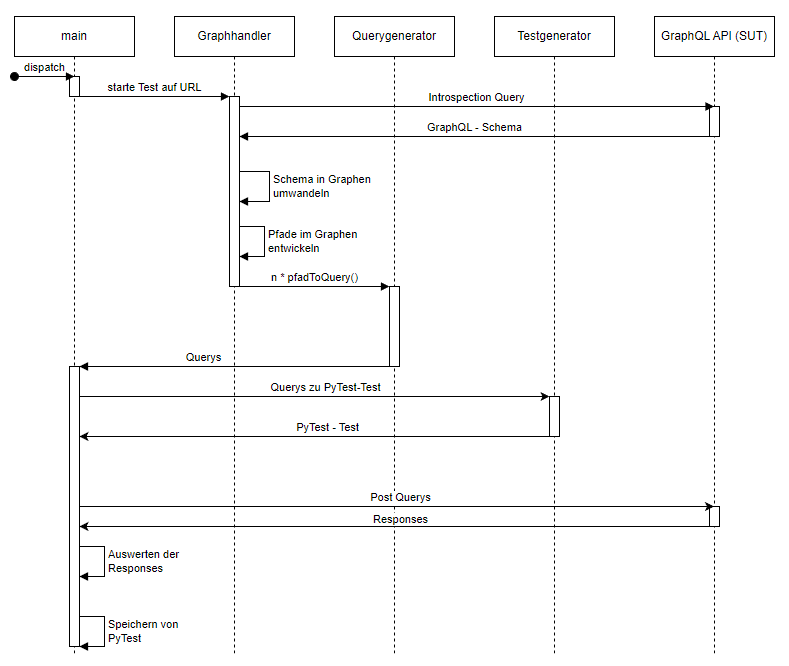
\includegraphics[width=\textwidth,height=\textheight,keepaspectratio]{img/sequenz}
\end{center}





